\section{Introduction}

\subsection{Docker setup}
\nblink{brats3D/01\_preprocess.ipynb}
correctly symblink files, execute container, copy out result file

\subsection{Zero out cubes}
\nblink{brats3D/02\_generate\_slices.ipynb}
iterate over everything, zero cubes

\begin{figure}[H]
\centering
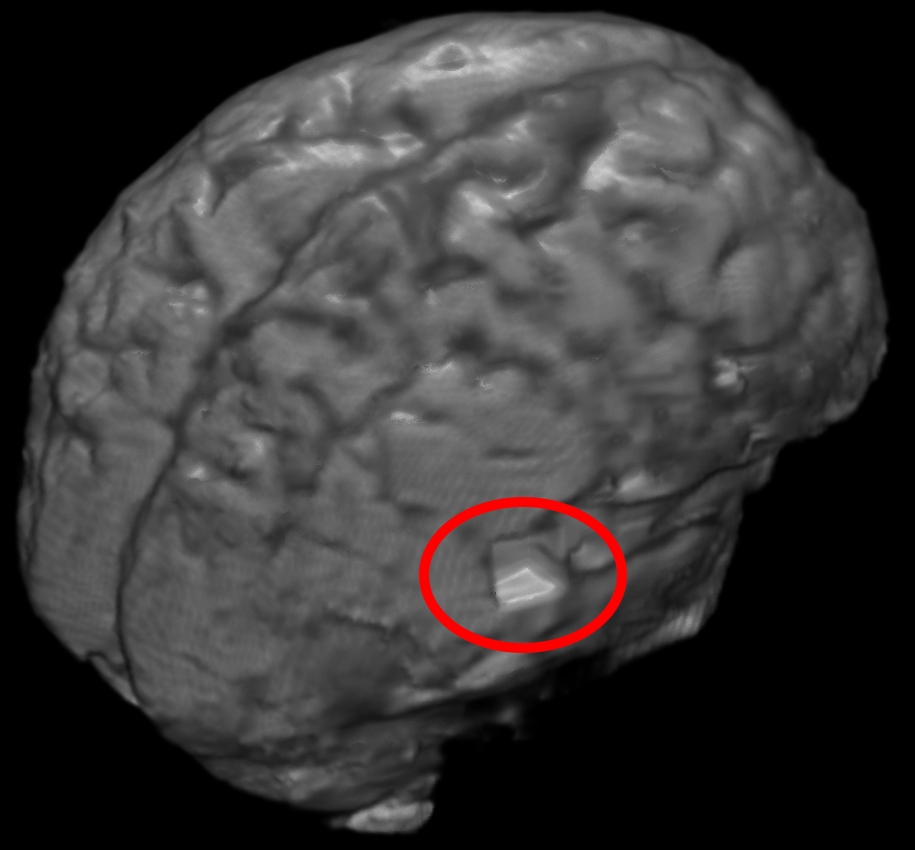
\includegraphics[width=10cm]{chapters/07_brats3d/images/brain-hdm-marked.png}
\caption{Modified scan with removed cube (red circle)}
\end{figure}


\subsection{Docker execution}
\nblink{brats3D/03\_execute.ipynb}
link up files

\subsection{Distance calculation}
\nblink{brats3D/04\_calculate\_hausdorff\_distance.ipynb}
hausdorff + MSE

\subsection{Visualization}
\nblink{brats3D/05\_display.ipynb}
We use cubes, do not bother with circles just upscale pixels

\subsection{High resolution single slice}
\nblink{brats3D/02a\_generate\_single\_slice.ipynb}
\nblink{brats3D/06\_display\_single\_slice.ipynb}

\subsection{Discussion}


\subsection{Conclusion}
